\documentclass[dvipdfmx]{jsbook}
\usepackage{mymacros}
\usepackage{amsmath,amssymb,amsthm}
\usepackage{mathrsfs}%花文字
\usepackage{tikz}
\theoremstyle{definition}
\newtheorem{dfn}{定義}[section]
\begin{document}
\タイトル{圏の練習1}{石塚 伶}
\section{Definition of category}
\begin{dfn}
\textbf{圏}(category) \category とは、以下のようなものをいう。
\end{dfn}
(1)\category の \textbf{対象}(obfect) と呼ばれるもの全体 Ob(\category)が与えられている。

$X$が圏\category の対象であるとき、$X \in \mathrm{Ob}(\mathscr{C})$のように表す。紛れのないときは、$X \in \mathscr{C}$のように略記する。

(2) \category の任意の二つの対象$X,Y$の間に、$X$から$Y$への\textbf{射}(morphism)または\textbf{矢}(arrow)の集合\category ($X,Y$)が与えられている。
\footnote{Mor($X,Y$)やHom($X,Y$)のように書くこともある。\category を明記するときには $\mathrm{Mor}_{\mathscr{C}} (X,Y) や  \mathrm{Hom}_{\mathscr{C}} (X,Y)$とも書く。}
射$f \in \mathscr{C}(X,Y)$を、
\[
X \overset{f}{\longrightarrow} Y
あるいは
f \colon X \longrightarrow Y
\]
のように表記する。
射は次の二つの性質を満たす。

(i)二つの射が次のように続いている場合、
\[
X \xlongrightarrow{f} Y \xlongrightarrow{g} Z
\]
これらの\textbf{合成}(composition)
$g \circ f \in \mathscr{C} (X,Z)$、つまり
\[ X \xlongrightarrow{g \circ f} Z \]
が与えられ、結合則を満たす。
すなわち、三つの射
\[
W \xlongrightarrow{e} X \xlongrightarrow{f} Y \xlongrightarrow{g} Z
\]
に対して、
$(g \circ f) \circ e = g \circ (f \circ e)$
が成立する。すなわち、
\[
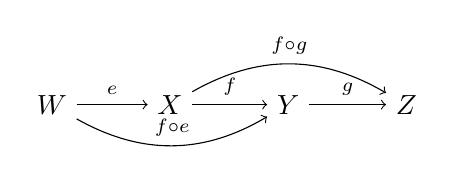
\begin{tikzpicture}[auto]
\node (w) at (0,0) {$W$}; \node (x) at (1.5,0) {$X$};
\node (y) at (3.0,0) {$Y$}; \node (z) at (4.5,0) {$Z$};
\draw[-to] (w) to node {$\scriptstyle e$} (x);
\draw[-to] (x) to node {$\scriptstyle f$} (y);
\draw[-to] (y) to node {$\scriptstyle g$} (z);
\draw[-to,bend left] (x) to node {$\scriptstyle f \circ g$} (z);
\draw[-to,bend right] (w) to node {$\scriptstyle f \circ e $} (y);
\end{tikzpicture}
\]
のように書ける。
こうして得られる等しい射を
$g \circ f \circ e$
と表す。
四つ以上の射の合成についても同様に表記する。

(ii) \category の任意の対象 $X$に対して、\textbf{恒等射}(identity)と呼ばれる射 $\mathrm{id}_X \in \mathscr{C} (X,Y)$がひとつずつ与えられており、合成に関し単位元的にふるまう。
すなわち、$X$からの任意の射
\[f \colon X \longrightarrow Y \]
に対して
$f \circ \mathrm{id}_{X} = f$
が成立し、$X$への任意の射
\[
e \colon W \longrightarrow X
\]
に対して
$\mathrm{id}_X \circ e = e$
が成立する。
$\mathrm{id}_X$をしばしば単に id と書く。あるいは、$1_X$ または単に$1$と書くこともある。
射$f \colon X \longrightarrow Y$に対して$X$を$f$の\textbf{始域}(domain)または\textbf{始点}(source)といい、$\mathrm{dom}f$や$s(f)$で表す。
また、$Y$を$f$の\textbf{終域}(codomain)または\textbf{終点}(target)といい、$\mathrm{cod}f$や$t(f)$で表す。
\end{document}


















.
